\chapter{Анализ предметной области, технологий стриминга и передачи видеоконтента для реализации серверной части системы} \label{ch1}

% не рекомендуется использовать отдельную section <<введение>> после лета 2020 года
%\section{Введение. Сложносоставное название первого параграфа первой главы для~демонстрации переноса слов в содержании} \label{ch1:intro}

	В данной главе проводится анализ предметной области работы, функциональности видеоплееров существующих стриминговых платформ, а также имеющихся решений в области хранения видеоконтента, и на основании полученных данных рассматриваются основные технологии для стриминга видео и области их применения, а также протоколы для передачи файлов на разном уровне взаимодействия: между клиентом и сервером и межсерверном. Целью данной главы является определение оптимальных технологий для реализации системы с долгосрочным доступ к видеоконтенту и поддержанием возможности его адаптивного воспроизведения на клиентской стороне.

\section{Анализ предметной области}

\subsection{Понятие видеостриминга}

	Цифровой мультимедийный контент охватывает широкий спектр цифровых данных, объединяющих текст, звук, изображения и видео, предоставляя пользователю разнообразные способы восприятия информации. С развитием информационных технологий цифровой контент стал важной частью жизни человека, включая интернет-платформы для хранения и распространения медиафайлов.

	Одним из ярких примеров является видеоконтент, который благодаря широкому распространению Интернета, мобильных устройств и быстрому развитию технологий передачи данных стал доступен большому числу пользователей по всему миру. С ростом спроса на видеоконтент возникла потребность в эффективных и удобных способах его доставки. Технологии видеостриминга, обеспечивающие бесперебойную передачу видео в реальном времени, стали одним из основных инструментов для решения этой задачи \cite{apostolopoulosVideoStreaming}. Эти технологии позволяют устранить необходимость в долгой загрузке файлов перед их воспроизведением, а также значительно облегчают доступ к контенту, позволяя обрабатывать контент на устройствах пользователей оптимально \cite{korotkovaMultimediaCommunication}.

	Видеостриминг делает возможным мгновенный доступ к видеоматериалам, что является важным фактором в эпоху, когда пользователи ожидают максимального удобства и скорости при получении информации.

	Видеостриминг — это технология передачи видеоконтента в режиме реального времени или по запросу, позволяющая воспроизводить видеофайлы по мере их загрузки . В отличие от традиционного скачивания, при котором необходимо дождаться полной загрузки файла перед его воспроизведением, видеостриминг обеспечивает более гибкий доступ к контенту. Это достигается путем разбиения видео на сегменты, которые последовательно передаются пользователю для декодирования и воспроизведения. Видеостриминг устраняет необходимость в загрузке файлов перед их просмотром, экономя время пользователей и пространство на их устройствах. Кроме того, видеостриминг решает проблему распределения контента. Он позволяет централизованно хранить видео на серверах и предоставить доступ к нему любому пользователю с подключением к интернету, устраняя географические ограничения \cite{apostolopoulosVideoStreaming}.
	
\subsection{Роль видеостриминга в различных сферах}

	Видеостриминг стал неотъемлемой частью различных сфер жизни, включая образование, бизнес, развлечения и социальные взаимодействия. Технологии потокового вещания предоставляют новые возможности для передачи информации в реальном времени и по запросу, что существенно влияет на коммуникацию и восприятие контента.

\textbf{Роль видеостриминга в образовании}

	В образовательной сфере видеостриминг позволяет проводить лекции, семинары и тренинги в режиме реального времени, обеспечивая доступ к знаниям независимо от географического положения участников \cite{brameEducationalVideos}. Это особенно актуально для дистанционного обучения и курсов повышения квалификации. Кроме того, видеостриминг дает возможность повысить вовлеченность студентов. Платформы, использующие видеостриминг, могут интегрировать различные элементы взаимодействия и навигации, которые помогают студентам повышать свою вовлечённость в учебный процесс. Более того, сам факт наличия функциональности навигации между видеоконтентом значительно увеличивает среднее время просмотра контента студентами \cite{brameEducationalVideos}, что говорит о необходимости их развития.

\textbf{Роль видеостриминга в коммерческой сфере}

	В коммерческой сфере видеоконтент, включая видеостриминг, также способствует значительному увеличению вовлеченности аудитории. В отличие от статичных рекламных материалов, видеоконтент является динамичным и визуально привлекательным, что позволяет удерживать внимание зрителей на протяжении более длительного времени \cite{ilyinaVideoMarketing}. Видеоконтент позволяет создавать живые презентации, обзоры, инструкции, которые значительно эффективнее передают информацию, чем текстовые или статичные изображения. Это способствует лучшему пониманию продукта и повышает вероятность совершения покупки. Кроме того, 60\% потребителей сначала обращают внимание на видеоконтент на веб-странице и только потом на текст или изображения. Также средний потребитель на 1200\% больше делится видеоконтеном, чем ссылками и текстами вместе взятыми \cite{ilyinaVideoMarketing}. На рисунке видно, что видеоконтент удерживает больше всего внимания пользователей по сравнению с другими представлениями информации. Видеостриминг в данном случае играет роль инструмента обеспечения качественного просмотра контента.

	\begin{figure}[ht!] 
		\center
		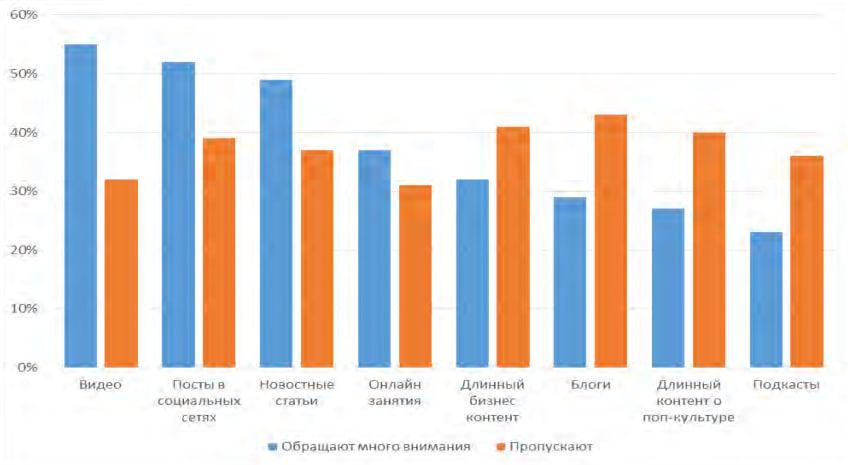
\includegraphics [scale=0.5] {my_folder/images//content_distribution}
		\caption{Распределение внимания пользователей между различными видами контента \cite{ilyinaVideoMarketing}}
		\label{fig:content_distribution}  
	\end{figure}

\subsection{Основные концепции видеостриминга}
	Ключевая особенность видеостриминга — это возможность доставки и воспроизведения контента практически в реальном времени. Традиционно стриминг используется для передачи как предварительно закодированных видеофайлов, так и живых трансляций. Однако существует ряд концепций видеостриминга, которые необходимо учитывать при разработке для обеспечения качественного воспроизведения контента \cite{apostolopoulosVideoStreaming}:

	\begin{itemize}[label=$\bullet$]
		\item Сжатие видео (Video Compression): видео требует больших объемов данных для хранения и передачи, что создает сложности при передаче через сети с ограниченной пропускной способностью, особенно для пользователей с медленным интернет-соединением. Сжатие видео позволяет уменьшить размер данных, сохраняя при этом приемлемое качество изображения;
		\item Адаптивный битрейт (Adaptive Bitrate Streaming): сетевые условия могут меняться в реальном времени, что приводит к снижению качества видео, если пропускная способность сети не соответствует требованиям для передачи высокого качества видеопотока. Эта концепция позволяет автоматически изменять качество видеопотока в зависимости от текущих сетевых условий;
		\item Протоколы потоковой передачи (Streaming Protocols): чтобы эффективно передавать видеопоток, необходимо синхронизировать передачу данных между сервером и клиентом, а также обеспечить управление потоком и контроль за его состоянием. Протоколы, соответствующие этому требованию, позволяют доставлять видео и аудио с минимальными задержкам при поддержки высокого качества передачи;
	\end{itemize}

	Соблюдение данных концепций является необходимым минимумом для реализации системы стриминга видео с высоким качеством.

\section{Анализ функциональности видеоплееров существующих стриминговых платформ}
	Стриминговые платформы активно развиваются, в том числе их технический и интерфейсный функционал. Быстрое развитие возможностей видеоплееров стремительно повышает качество взаимодействия с пользователями, что приводит к увеличению вовлеченности зрителей. Эта вовлеченность является ключевым элементом для монетизации контента, через рекламу или другие механизмы, напрямую влияя на прибыль стриминговых сервисов \cite{xiaoShortVideoMarketing}.

	Для анализа существующих стриминговых платформ стоит рассматривать те, которые имеют наибольший срок эксплуатации и стабильный спрос. Это обусловлено тем, что они не только предлагают проверенные временем технологии, но и формируют тренды в области функционала, которые улучшают пользовательский опыт. Среди таких платформ можно выделить YouTube и Twitch, которые являются лидерами в своей категории и на протяжении многих лет задают стандарты в области потокового видео. Из базовых функций, которые содержат плееры всех перечисленных платформ можно выделить:
	
	\begin{enumerate}[1.]
		\item Управление воспроизведением:
			\begin{itemize}[label=$\bullet$]
				\item Кнопки воспроизведения и паузы: стандартные кнопки для начала и приостановки воспроизведения видео;
				\item Перемотка по времени: возможность перематывать видео по временной шкале плеера. Прокрутка осуществляется с точностью до нескольких секунд, что позволяет быстро перемещаться по видео;
				\item Управление громкостью: встроенная регулировка громкости с помощью ползунка, а также кнопка для выключения звука.
			\end{itemize}
		\item Полноэкранный режим: возможность развернуть видео на весь экран, что улучшает восприятие контента;
		\item Регулировка скорости воспроизведения: плеер дает возможность замедлять или ускорять видео, регулируя скорость воспроизведения (например, 0.5x, 1x, 1.5x, 2x);
		\item Поддержка доступности и отзывчивого интерфейса: плеер адаптирован под различные устройства, включая мобильные телефоны, планшеты и компьютеры.
	\end{enumerate}
	
	Из платформенных особенностей можно выделить наличие у плеера YouTube субтитров на разных языках, созданных предварительно с помощью технологий машинного обучения, а также график интерактивной популярности, характеризующий, какие части видео пользователи чаще всего просматривают, перематывают или возвращаются к ним. Платформа Twitch, помимо перечисленного выше функционала, содержит интерактивные виджеты для проведения опросов разного типа, однако такая функциональность актуальна только для видеостриминга в режиме реального времени, так как выполняет роль коммуникации между автором и пользователями в процессе производства и потребления контента. Интерфейс видеоплееров рассмотренных платформ представлен на рисунках 2-3.
	Все перечисленные платформы предоставляют пользователям схожие базовые возможности для работы с видеоконтентом. Однако создание контента становится всё более сложным процессом, поскольку авторы действуют в условиях высокой конкуренции и вынуждены разрабатывать новые подходы к его производству. Сегодня популярным становится использование нескольких камер или видеопотоков, особенно в таких сферах, как образование, медицина или индустрия развлечений и медиа, где требуется передавать пользователю одновременно несколько видеопотоков, например, для отображения полной картины о проведении хирургической операции. Тем не менее, текущие платформы предоставляют возможность воспроизведения контента преимущественно в одном потоке. Управление отображением нескольких элементов видео осуществляется авторами посредством монтажа. Это ограничение накладывает дополнительные требования на процесс создания видео и не всегда позволяет в полной мере отразить потенциал современных методов производства контента.
	Для удовлетворения потребностей таких авторов и улучшения пользовательского опыта внедрение поддержки воспроизведения видео в нескольких синхронизированных потоках на уровне платформы позволило бы повысить вовлечённость пользователей за счёт большего выбора и гибкости в просмотре контента. В связи с этим в рамках данной работы будет разработано приложение, реализующее эту функциональность.
	Однако для реализации таких возможностей на клиентской стороне необходимо также, чтобы на стороне сервера поддерживались адаптивность стриминга, технологии сжатия и хранения видео, а также возможность сегментированной загрузки контента для авторов. Эти требования обеспечивают качественное воспроизведение видео для пользователей, даже при низкой пропускной способности сети, и для авторов контента, так как позволяют целостно загружать видео без потери данных и с возможностью восстановления сессий загрузки.

\section{Анализ существующих решений в области хранения видеоконтента}
	Хранение больших объемов бинарных данных (blob) при разработке системы с распределённой загрузкой контента является технически нетривиальной задачей, требующей эффективного управления большими объемами данных. Важно учитывать вопросы масштабируемости, скорости доставки и безопасности. Для решения этих проблем необходимо провести анализ современных решений в этой области и заимствовать лучшие практики, чтобы создать оптимальную архитектуру системы.

	\textbf{Amazon Web Services}
	
	Amazon web Services (AWS) - один из старейших игроков на рынке облачных технологий, основанный в 2006 году. Он предоставляет широкий спектр компьютерных услуг, таких как облачные хранилища, службы баз данных, аналитика, сетевые сервисы и многое другое \cite{muftiCloudReview}.

	AWS состоит из компонентов перечисленных ниже:
	\begin{itemize}[label=$\bullet$]
		\item Amazon CloudFront: этот сервис предназначен для доставки контента, используемого на веб-сайтах. Он поддерживает как статические, так и динамические данные, а также потоковое видео. CloudFront использует распределенную сеть серверов по всему миру для оптимизации доставки контента пользователям;
		\item Балансировка нагрузки (Load Balancing): балансировка нагрузки позволяет повысить эффективность работы серверов и приложений. Это важный элемент сетевой инфраструктуры, который улучшает архитектуру классических веб-приложений. В AWS трафик распределяется между экземплярами сервисов, размещенными на разных ресурсах. При этом нагрузка также корректируется в зависимости от добавления или удаления экземпляров сервиса из балансировщика;
		\item Amazon RDS (Amazon Relational Database Service): сервис Amazon RDS предоставляет возможность работы с реляционными базами данных, аналогичными MySQL или Microsoft SQL, обеспечивая доступ к базе данных в облаке с удобным управлением и настройкой;
		\item Эластичный кэш (Elastic Cache): система управления кэшированием в облаке, которая обеспечивает эффективную работу за счет сокращения нагрузки на серверы. Она помогает оптимизировать использование памяти и снижать нагрузку на сервисы, улучшая их надежность;
		\item Простой сервис очередей (Simple Queue Service): облачный сервис для асинхронного обмена сообщениями между компонентами распределенных систем. Обеспечивает надежную доставку, масштабируемость, поддержку стандартных и FIFO очередей, а также интеграцию с другими сервисами AWS. Позволяет снизить связность компонентов, оптимизировать производительность и управлять нагрузкой на системы.
	\end{itemize}

	\textbf{Яндекс.Облако}

	Яндекс.Облако — это набор взаимосвязанных сервисов и инструментов для работы в облачной платформе \cite{migratovYandexCloud}. Это платформа является отечественной и предоставляет для клиентов сервисы и инструменты, решающие те же проблемы, что и составляющие части AWS. Яндекс. Облако состоит из компонентов перечисленных ниже \cite{yandexDocs}:

	
	\begin{itemize}[label=$\bullet$]
		\item Объектное хранилище (Object Storage): этот сервис представляет собой масштабируемое хранилище для объектов данных, которое подходит для хранения любых типов файлов;
		\item Управляемые базы данных (Managed Databases): этот компонент включает поддержку PostgreSQL, MySQL, MongoDB, Redis, ClickHouse, Elasticsearch и других баз данных. Это решение похоже на AWS RDS;
		\item Load Balancers (Network/Application): Балансировщики нагрузки для распределения трафика между серверами, аналогичные AWS Load Balancing;
		\item Очереди сообщений (Message Queue): сервис позволяет организовать асинхронный обмен сообщениями между компонентами системы, аналогичен Amazon SQS.
	\end{itemize}

	И Yandex.Cloud, и AWS предоставляют мощные и гибкие решения для хранения, обработки и передачи больших бинарных объектов, которые обеспечивают высокую надежность, масштабируемость и интеграцию с другими сервисами. Однако их использование несёт в себе ряд определённых рисков и ограничений при разработке рассматриваемой в ходе работы системы, так как обе платформы работают на основе подписки или оплаты за использование, что делает их применение оправданным только для проектов с достаточным финансовым бюджетом, оба решения являются проприетарными и не предоставляют доступа к исходному коду, что ограничивает гибкость настройки и прозрачность. В связи с этим для решения поставленных в ходе работы задач оптимальным выбором будет реализовать платформу для хранения контента самостоятельно на основе следующих компонентов: балансировщики нагрузки, очереди сообщений, объектное хранилище, управляемые базы данных, управляемые базы данных для кэширования.
	

\section{Технологии стриминга видео} \label{ch1:sec1}

	Стриминг позволяет передавать видеоконтент в виде пакетов данных, что обеспечивает воспроизведение мультимедиа ещё до завершения загрузки файла. Такой подход снижает задержки перед началом просмотра и уменьшает требования к объему хранилища на стороне пользователя \cite{apostolopoulosVideoStreaming}. 
	
	Стриминг решает проблему распределения сетевой и вычислительной нагрузки не только на стороне клиента, но и на стороне сервера. Кроме того, использование технологий стриминга хорошо согласуется с микросервисной архитектурой приложений и позволяет без затруднений горизонтально масштабировать раздачу видеоконтента - увеличивать количество реплик сервисов, отвечающих за хранение и передачу контента пользователям при соответствующих запросах. 

	Технологии стриминга можно разделить на следующие категории \cite{apostolopoulosVideoStreaming}:
	\begin{itemize}[label=$\bullet$]
		\item Способ кодирования:
			\begin{itemize}[label=$\circ$]
				\item В реальном времени (Real-time encoding);
				\item Предварительное (Pre-encoded video).
			\end{itemize}
		\item Тип связи:
			\begin{itemize}[label=$\circ$]
				\item Точка-точка (Point-to-point);
				\item Многовещание (Multicast);
				\item Широковещание (Broadcast).
			\end{itemize}
		\item Скорость передачи данных:
			\begin{itemize}[label=$\circ$]
				\item Постоянная (Constant Bit Rate, CBR);
				\item Переменная (Variable Bit Rate, VBR).
			\end{itemize}
		\item Описание потока:
			\begin{itemize}[label=$\circ$]
				\item Одиночное описание (Single Description Coding, SD);
				\item Множественное описание (Multiple Description Coding, MD).
			\end{itemize}
		\item Протокол передачи данных:
			\begin{itemize}[label=$\circ$]
				\item TCP;
				\item UDP.
			\end{itemize}
		\item Тип стриминга:
			\begin{itemize}[label=$\circ$]
				\item Прямой эфир (Live streaming);
				\item Видео по запросу (On-demand streaming).
			\end{itemize}
		\item Адаптивность:
			\begin{itemize}[label=$\circ$]
				\item Адаптивный стриминг (Adaptive streaming);
				\item Неадаптивный стриминг (Non-adaptive streaming).
			\end{itemize}
	\end{itemize}
	
	Технологии стриминга видео, которые будут использованы в системе, определяются на основе решаемых задач, так как каждая из них соответствует определённым критериям. Иными словами, выбор технологий должен опираться на их соответствии этим критериям для обеспечения наиболее эффективного решения. Основными критериями для реализации рассматриваемой в ходе работы системы являются:

	
	\begin{itemize}[label=$\bullet$]
		\item Способ кодирования: предварительное - система должна поддерживать долгосрочный доступ к видеоконтенту, а не доступ к контенту в реальном времени;
		\item Тип связи: точка-точка - в системе связь осуществляется между двумя конечными точками — сервером и клиентом;
		\item Скорость передачи данных: переменная - каждый видеопоток должен быть адаптивен и менять битрейт в зависимости от динамичности контента;
		\item Описание потока: одиночное - видеопоток может быть представлен в виде одного файла со списком сегментов, каждый из которых может быть получен клиентом по запросу;
		\item Протокол передачи данных: TCP - система предоставляет долгосрочный доступ к контенту, все сегменты видео хранятся на сервере и являются целостными, поэтому должны доставляться пользователю без потерь;
		\item Тип стриминга: видео по запросу;
		\item Адаптивность: адаптивный стриминг - система должна иметь возможность регулировать качество воспроизведения видео на стороне пользователя в зависимости от индивидуальной скорости передачи данных.
	\end{itemize}


\subsection{Протокол RTP}

	RTP предоставляет функции транспортировки данных в реальном времени от источника до получателя, подходящие для приложений, передающих данные в реальном времени, такие как аудио, видео или данные моделирования, через мультикаст или юникаст-сети \cite{rfcRtp}.

	Мультикаст-сети (Multicast) используются для отправки одного потока данных нескольким получателям одновременно.

	Юникаст-сети (Unicast) предполагает индивидуальную передачу данных от отправителя к каждому получателю. Для каждого клиента создаётся уникальный поток.

	Каждый RTP-пакет содержит фиксированный заголовок, за которым следует полезная нагрузка переменной длины. Заголовок включает информацию, необходимую для синхронизации и демультиплексирования медиапотоков \cite{rfcRtp}. Формат заголовка представлен на рисунке \cite{rfcRtp}.

	\begin{figure}[ht!] 
		\center
		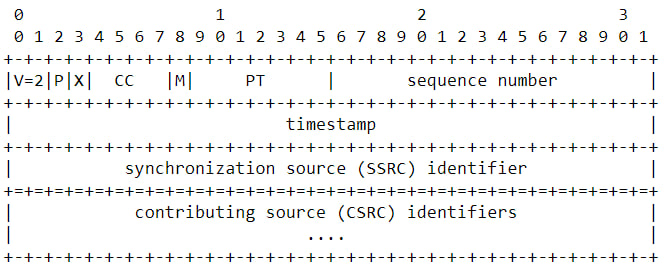
\includegraphics [scale=0.8] {my_folder/images//rtp_headers}
		\caption{Заголовок RTP-пакета \cite{rfcRtp}}
		\label{fig:rtp_headers}  
	\end{figure}

	RTP использует переменную скорость передачи данных в зависимости от характеристик медиа и сети. Этот протокол также обычно использует одно описание потока для мультимедийных данных, где каждый поток определяется отдельно для синхронизации. В качестве протокола для передачи данных используется UDP, так как он предназначен для приложений с низкими задержками и реального времени - целостность данных не играет ключевой роли, допустимы небольшие потери пакетов. RTP поддерживает адаптивный стриминг с использованием RTCP, который предоставляет отчеты о состоянии сети. Это позволяет адаптировать видеопоток \cite{rfcRtp}.

\subsection{Стандарт MPEG-DASH}

	MPEG-DASH (Dynamic Adaptive Streaming over HTTP) — это стандарт для эффективной потоковой передачи мультимедийных данных с использованием существующей инфраструктуры HTTP. Он поддерживает как потоковую передачу по запросу (on-demand), так и в реальном времени (live streaming) \cite{mpegDashSite}.

	Этот стандарт разделяет видео и аудио контент на небольшие сегменты, каждый из которых может быть закодирован с разным битрейтом. Также он поддерживает возможность определения длины сегмента по времени, что крайне удобно для выбора оптимального значения при запуске, например, A/B экспериментов для приложений, использующих эту технологию. Без использования средств нагрузочного тестирования - только на основе различий в продуктовых и технических метриках между двумя версиями приложения можно определить оптимальное значение длины сегмента.

	Воспроизведение начинается с загрузки первого сегмента, после чего плеер динамически выбирает сегменты с оптимальным качеством в зависимости от текущей скорости сети и возможностей устройства. MPEG-DASH не зависит от кодеков, что позволяет использовать различные форматы сжатия: H.264, H.265, VP8 и другие. Стандарт использует в качестве протокола передачи данных на прикладном уровне HTTP, на транспортном - TCP \cite{sodagarMpegDash}.
	
	Важно отметить, что использование протоколов HTTP и TCP в основе стандарта позволяет поддерживать целостность передаваемых пользователю сегментов, что влечёт за собой определённые накладные расходы при передаче данных, но лучше всего подходит для стриминга видео по запросу, так как улучшает пользовательский опыт в системах с долгосрочным доступом к контенту.
	
	Стандарт поддерживает как потоковое вещание по запросу, так и прямые трансляции (live streaming), включая функции перемотки назад и паузы в прямом эфире. Представление видеопотока описывается в файле формата MPD. Файл MPD (Media Presentation Description) содержит структуру мультимедийного контента, включая информацию о сегментах, их длительности, битрейте, разрешении и других параметрах. MPD может быть статическим или динамическим, в зависимости от типа контента \cite{sodagarMpegDash}.

\subsection{Протокол HLS}

	HTTP Live Streaming (HLS) — это протокол адаптивной потоковой передачи мультимедийного контента, разработанный компанией Apple, который используется для доставки мультимедийного контента по сети Интернет \cite{rfcHls}.
	
	HLS поддерживает потоковую передачу в реальном времени, где данные кодируются и сегментируются для прямых трансляций сразу при получении данных и передаёт их пользователю.
	
	Этот протокол также поддерживает передачу заранее закодированных видео по запросу пользователя. Предварительно созданные и закодированные сегменты упрощают доставку пользователю и минимизируют задержки. Основной режим работы HLS — это точка-точка, где клиент напрямую запрашивает сегменты через HTTP у сервера. Протокол изначально не поддерживает многовещание или широковещание \cite{rfcHls}. Для работы с такими режимами требуется дополнительная инфраструктура (например, использование CDN).
	
	HLS позволяет использовать переменный битрейт. Клиент адаптируется к доступной пропускной способности, выбирая поток с соответствующим качеством. Это позволяет оптимизировать использование сети. Протокол также теоретически поддерживает постоянный битрейт, однако особое внимание в протоколе уделяется именно переменному битрейту. HLS работает исключительно через HTTP, а значит, поверх TCP. Это обеспечивает целостность данных при передаче \cite{rfcHls}. HLS использует единую последовательность сегментов, которые представляют поток на определённом уровне качества \cite{fecheyrHlsReview}. Его можно отнести к одиночному типу описания потока.
	
	Так как протокол был создан компанией Apple, он занимает доминирующее положение в её продуктах, в частности, в мобильной и веб версиях браузера Safari. HLS поддерживается по умолчанию в этом браузере и не требует установки дополнительной инфраструктуры для использования, что выделяет её среди остальных технологий, когда речь идёт о продуктах Apple.
	
	Концептуально HLS состоит из трёх частей: серверного компонента, компонента раздачи и клиентского программного обеспечения \cite{fecheyrHlsReview}. Архитектура протокола представлена на рисунке \ref{fig:hls_architecture}.

	\begin{figure}[ht!] 
		\center
		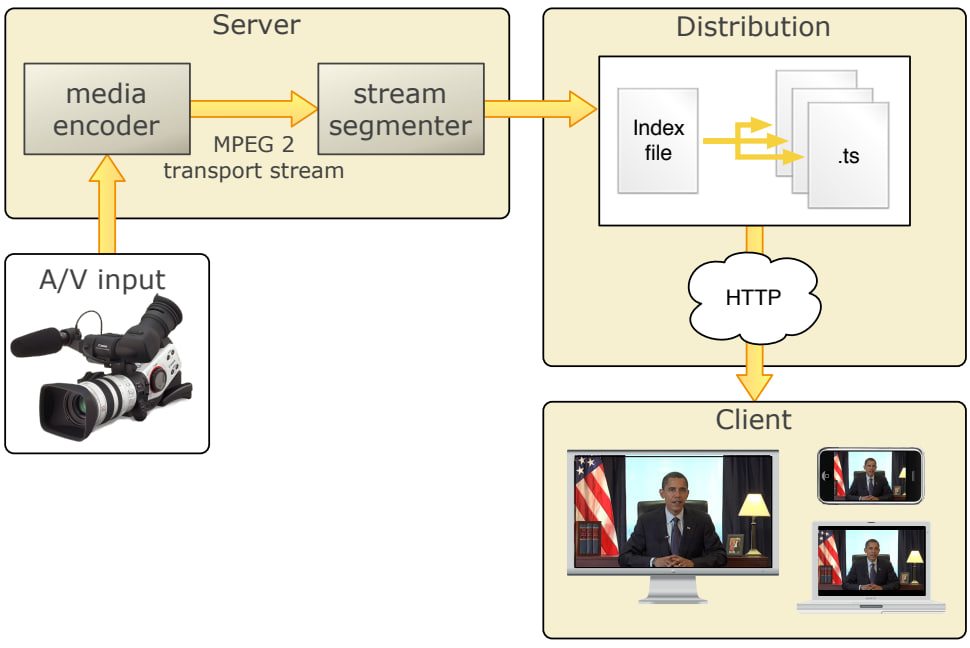
\includegraphics [scale=0.6] {my_folder/images//hls_architecture}
		\caption{Архитектура протокола HTTP Live Streaming \cite{fecheyrHlsReview}} 
		\label{fig:hls_architecture}  
	\end{figure}

\subsection{Сравнительный анализ технологий стриминга видео}

	Для выбора оптимального решения стриминга видео с долгосрочным доступом к контенту необходимо сравнить определённые ранее технологии по выделенным в разделе 1.2 критериям. Рассмотрим таблицу \ref{fig:streaming_compare}.

	\begin{table} [htbp]% Пример оформления таблицы
		\centering\small
		\caption{Сравнение технологий стриминга видео}%		
		\begin{tabular}{|p{3.5cm}|p{3.5cm}|p{3.5cm}|p{3.5cm}|}
			\hline
			Критерий сравнения&RTP&MPEG-DASH&HLS\\
			\hline
			Способ кодирования&Реальное время (Real-time)&Предварительное (Pre-encoded) и Реальное время (Real-time)&Предварительное (Pre-encoded)\\ \hline
			Тип связи&Точка-точка (Point-to-point), Многовещание (Multicast)&Точка-точка (Point-to-point)&Точка-точка (Point-to-point)\\ \hline
			Скорость передачи данных&Переменная (VBR)&Переменная (VBR), Постоянная (CBR)&Переменная (VBR), Постоянная (CBR)\\ \hline
			Описание потока&Множественное (MD)&Одиночное (SD)&Одиночное (SD)\\ \hline
			Протокол передачи данных&UDP&TCP&TCP\\ \hline
			Тип стриминга&Прямой эфир&Видео по запросу, Прямой эфир&Видео по запросу, Прямой эфир\\ \hline		
			Адаптивность&Неадаптивный стриминг&Адаптивный стриминг&Адаптивный стриминг\\ \hline		
		\end{tabular}	
		\label{fig:streaming_compare}
		\normalsize% возвращаем шрифт к нормальному
	\end{table}
	
	Таблица выше показывает, что для долгосрочного доступа к видеоконтенту наиболее подходящими решениями являются HLS и MPEG-DASH. Обе технологии поддерживают переменный битрейт, благодаря чему возможен адаптивный стриминг. Они используют протокол TCP, что гарантирует целостность данных при передаче. Эти протоколы позволяют получить видео по запросу и обеспечивают качественный пользовательский опыт на разных устройствах.
	
	В качестве основной технологии для стриминга видео явно стоит выделить MPEG-DASH. Помимо остальных преимуществ, эта технология позволяет более качественно минимизировать задержки при передаче данных, благодаря более атомарному разбиению видео на сегменты \cite{bouzakariaLowLatencyDash}. Однако для разных версий браузера Safari стоит отдать предпочтение протоколу HLS. Инфраструктура этого браузера оптимизирована именно для работы с HLS. Таким образом, для поддержки кроссплатформенности рассматриваемой в ходе работы системы наилучшим решением будет использовать и MPEG-DASH, и HLS, но для разных браузерных окружений. Загрузку инфраструктуры MPEG-DASH необходимо производить только при отсутствующей поддержке HLS.

\section{Протоколы для передачи файлов между узлами сетей}
	При выборе протокола в системах с загрузкой и передачей файлов между узлами сети важно учитывать особенности видеоконтента, который отличается большим объемом и требует продуманного подхода. Различные протоколы предлагают решения в зависимости от задач: одни оптимизированы для передачи небольших сегментов, другие обеспечивают целостность и надежность при отправке крупных файлов. Также важно учитывать безопасность системы и кроссплатформенность технологии на клиентской стороне.

\subsection{Протокол HTTP}
	HTTP (HyperText Transfer Protocol) — это протокол передачи гипертекстовых документов, который является основным способом обмена данными в интернете \cite{rfcHttp10}. HTTP был разработан для обмена текстовыми документами и ресурсами между веб-серверами и клиентами, однако со временем он стал основным механизмом для передачи данных любых типов, включая файлы или бинарные данные.
	
	Основные принципы работы HTTP:
	\begin{itemize}[label=$\bullet$]
		\item HTTP представляет собой протокол прикладного уровня модели OSI (Open Systems Interconnection). Он работает в модели запрос-ответ, где клиент (обычно это веб-браузер) отправляет запрос к серверу, а сервер в ответ отправляет данные;
		\item Каждый HTTP запрос состоит из:
		\begin{itemize}[label=$\circ$]
			\item Метод запроса (GET, POST, PUT, DELETE и др.);
			\item URL (Uniform Resource Locator) — адрес ресурса;
			\item HTTP-версия (например, HTTP/1.1);
			\item Заголовки — дополнительные метаданные, которые могут содержать информацию о клиенте \cite{gourleyHttpGuide}. Заголовки можно использовать для передачи данных о текущей пользовательской сессии в зашифрованном виде, а также для разметки сегментов файлов при их загрузке в виде бинарных данных;
			\item Тело запроса — данные, передаваемые с запросом.
		\end{itemize}
	\end{itemize}

	Пример взаимодействия между сервером и клиентом на основе протокола HTTP представлена на рисунке \ref{fig:http_scheme}.
	\begin{figure}[ht!] 
		\center
		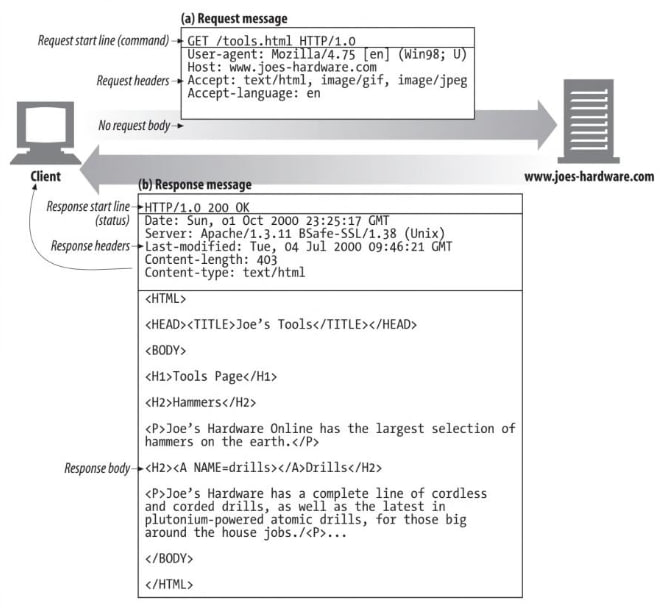
\includegraphics [scale=0.8] {my_folder/images//http_scheme}
		\caption{Пример взаимодействия между сервером и клиентом на основе протокола HTTP \cite{gourleyHttpGuide}}
		\label{fig:http_scheme}  
	\end{figure}
	
	Рассмотрим различные способы передачи файл на сервер с помощью HTTP:
	\begin{itemize}[label=$\bullet$]
		\item Одним из самых распространенных способов отправки файлов через HTTP является использование заголовка "Content-Type" со значением "multipart/form-data" \cite{rfcHttp10}. Он используется в основном при отправке данных через HTML-формы, когда помимо файлов могут быть отправлены другие типы данных, такие как текстовые поля;
		\item Файлы можно передавать в виде бинарных данных. Как и в предыдущем способе, для передачи используется заголовок "Content-Type", но со значением "application/octet-stream". Этот подход обычно используется для передачи больших файлов или когда необходимо передать двоичные данные, такие как изображения или видео. Преимущество данного способа неочевидно, однако он позволяет разбивать файл на клиентской стороне на несколько сегментов и отправлять его в виде нескольких частей. Разметку для этих сегментов можно передавать в заголовках запроса;
		\item Файлы могут быть закодированы в строку Base64 и отправлены в виде строки. Например, в теле запроса или в качестве части данных JSON. Такой способ не подходит для передачи больших файлов, так как требует дополнительных неэффективных вычислений на клиентской и серверной сторонах.
	\end{itemize}

	Преимущества использования протокола при загрузке файлов:
	\begin{itemize}[label=$\bullet$]
		\item Кроссплатформенность и поддержка всех браузеров позволяет передавать файлы с различных устройств и браузерных сред;
		\item HTTP позволяет отправлять файлы различными способами и предоставляет большую гибкость в формировании запросов к серверу благодаря наличию заголовков. Файлы можно предварительно разбить на сегменты на клиентской стороне и последовательно или параллельно отправлять на сервер;
		\item HTTP в совокупности с протоколом SSL/TLS позволяют обеспечить защищённое шифрованное соединение между клиентом сервером. Совокупность этих протоколов обобщённо имеет название HTTPS. HTTPS поддерживается по умолчанию всеми современными браузерами и не требует дополнительных настроек в отличие от других протоколов.
	\end{itemize}
	
	 Недостатки использования протокола при загрузке файлов:
	\begin{itemize}[label=$\bullet$]
		\item Cпецификация HTTP не ограничивает размер запроса, однако серверы и браузеры могут накладывать ограничения на размер передаваемых данных \cite{rfcHttp10}. В таком случае файл необходимо предварительно обработать на стороне клиента и отправлять данные несколькими запросами в виде, например, сегментов;
		\item При отправке больших файлов HTTP-запросы могут сильно загружать сервер, так как загрузка файлов без предварительного преобразования на клиентской стороне требует их синхронной обработки на стороне сервера;
		\item Если передача файла занимает много времени, могут возникать проблемы с тайм-аутами на стороне клиента или сервера. Тайм-ауты могут возникать, если сервер или клиент не получают данных в течение установленного времени.
	\end{itemize}

\subsection{Протокол FTP}
	FTP - это протокол, разработанный для надежной передачи файлов
	между клиентами и серверами в сетях с использованием TCP \cite{rfcFtp}.
	
	Основные цели и задачи протокола FTP:
	\begin{itemize}[label=$\bullet$]
		\item Перенос файлов: обеспечение механизма для передачи файлов между хостами, независимо от их операционных систем или файловых структур \cite{rfcFtp};
		\item Абстракция файловой структуры: протокол предоставляет общий интерфейс для работы с файлами \cite{rfcFtp}, скрывая различия в файловых системах между клиентом и сервером;
		\item Поддержка взаимодействия человека с системой: FTP предлагает удобный способ работы для клиента, предоставляя команды для взаимодействия с сервером через текстовые запросы;
	\end{itemize}
	
	Особенности протокола:
	\begin{itemize}[label=$\bullet$]
		\item FTP использует два независимых соединения \cite{rfcFtp}:
		\begin{itemize}[label=$\circ$]
			\item Управляющее соединение (Control Connection): работает на 21 TCP-порту и используется для передачи команд и ответов между клиентом и сервером \cite{rfcFtp};
			\item Соединение данных (Data Connection): работает на 20 TCP-порту и используется непосредственно для передачи файлов каталогов.
		\end{itemize}
		\item Режимы передачи данных:
		\begin{itemize}[label=$\circ$]
			\item Активный режим (Active Mode): сервер открывает соединение для передачи данных на указанный клиентом адрес \cite{rfcFtp};
			\item Пассивный режим (Passive Mode): сервер сообщает клиенту о доступном порте, и клиент инициирует соединение \cite{rfcFtp}.
		\end{itemize}
	\end{itemize}
	
	Преимущества FTP:
	\begin{itemize}[label=$\bullet$]
		\item Протокол предоставляет команды для работы с файлами и каталогами: создание, удаление, переименование и перемещение;
		\item TCP, который использует FTP, гарантирует доставку всех пакетов \cite{rfcFtp};
		\item FTP поддерживает возобновление передачи файлов \cite{rfcFtp};
		\item Протокол обеспечивает универсальный подход для передачи как текстовых, так и двоичных данных.
	\end{itemize}
	
	Ограничения и недостатки FTP:
	\begin{itemize}[label=$\bullet$]
		\item Логины, пароли и данные передаются в незашифрованном виде \cite{rfcFtp}. Необходимо самостоятельно поддерживать шифрование на серверной и клиентской частях приложения;
		\item Протокол не поддерживает современные механизмы авторизации, такие как токены;
		\item Не поддерживается в современных браузерах.
	\end{itemize}

\subsection{Сравнительный анализ протоколов передачи файлов между узлами сетей}	
	Ключевым требованием к протоколу для передачи файлов между клиентом и сервером является его кроссплатформенность. Из рассмотренных в данной главе протоколов этому требованию соответствует только протокол HTTP. Кроме того, вместе с этим протоколом во всех современных браузерах по умолчанию поддерживается также SSL/TLS \cite{rfcHttp10}, что обеспечивает безопасность передаваемых пользователем данных. Поэтому в качестве протокола для передачи данных между сервером и клиентом оптимальным выбором является HTTP.
	
	В системах хранения и обработки видео зачастую используются разные серверы для выполнения этих функций в отдельности. Для передачи файлов между сервером обработки и сервером хранения также необходимо сделать выбор в пользу того или иного протокола. В данном случае нет необходимости беспокоиться о его поддержке, так как клиенты протокола можно установить на соответствующие сервера. Кроме того, сеть передачи между ними можно виртуализировать и скрыть от внешнего пользователя, на сегодняшний день с этим отлично справляются средства контейнеризации Docker, containerd, и другие. Это позволяет обеспечить безопасность между серверами, поэтому средства авторизации и аутентификации самого протокола играют посредственную роль. Таким образом, для межсерверного обмена файлами подходит не только протокол HTTP, но и FTP. Благодаря своему двухканальному режиму, более развёрнутому списку команд для работы с файлами и директориями, а также возобновлению сессий загрузки FTP является наиболее эффективным решением для межсерверного обмена файлами.

\section{Выводы}
	В данной главе были рассмотрены предметная область проекта, включая технологии стриминга  и передачи видеоконтента для реализации серверной части системы. Проведён сравнительный анализ производительности, адаптивности и совместимости с современными браузерами соответствующих технологий.

	По итогам сравнительного анализа были сделаны следующие выводы:
	\begin{enumerate}[label=$\bullet$]
		\item Для стриминга видео целесообразно использовать протоколы MPEG-DASH и HLS, которые обеспечивают адаптивный стриминг, минимальные задержки и целостность данных при передаче. На серверной части системы необходимо поддерживать оба протокола, а на клиенте - в зависимости от браузерной среды: MPEG-DASH подходит для большинства браузеров, кроме Safari - для него более предпочтителен HLS;
		\item В качестве кодека для сжатия видео выбран H.264, так как он демонстрирует лучшее качество сжатия при меньших битрейтах, высокую производительность, поддержку аппаратного декодирования и совместимость с современными устройствами и протоколами;
		\item Для передачи данных между клиентом и сервером выбран HTTP, благодаря его кроссплатформенности, поддержке шифрования (с использованием SSL/TLS) и гибкости работы с сегментированной передачей данных. Для межсерверного обмена контентом был выбран FTP, который обеспечивает надёжную передачу файлов с возможностью возобновления загрузок.
	\end{enumerate}

	